\documentclass[first=dgreen,second=purple,logo=yellowexc]{aaltoslides}
%\documentclass{aaltoslides} % DEFAULT
%\documentclass[first=purple,second=lgreen,logo=redque,normaltitle,nofoot]{aaltoslides} % SOME OPTION EXAMPLES


\usepackage[latin9]{inputenc}
\usepackage[T1]{fontenc}
\usepackage{amssymb}
\usepackage{amsmath}
\usepackage{url}
\usepackage{lastpage}
\usepackage{lastpage}
\usepackage{multirow}
\usepackage{colortbl}
\usepackage{comment}
\usepackage{algorithm}
\usepackage{algorithmic}
\usepackage{stmaryrd}
\usepackage{bm}
\usepackage{natbib}
\usepackage[SCI,RGB]{aaltologo} % RGB, Coated, Uncoated
\usepackage{multicol}

\newcommand{\var}{\textbf{Var}}
\newcommand{\cov}{\textbf{Cov}}
\newcommand{\ip}[2]{\langle #1, #2 \rangle}
\newcommand{\sets}[1]{\{#1\}}
\newcommand{\ind}[1]{{\boldsymbol{1}}_{\sets{#1}}}
\newcommand{\Ecal}{\mathcal{E}}
\newcommand{\Acal}{\mathcal{A}}
\newcommand{\Fcal}{\mathcal{F}} %feature space
\newcommand{\Gcal}{\mathcal{G}}
\newcommand{\Hcal}{\mathcal{H}} %feature space / RKHS
\newcommand{\Ncal}{\mathcal{N}} %covering numbers
\newcommand{\Pcal}{\mathcal{P}} %Family Probability
\newcommand{\Xcal}{\mathcal{X}} %set of possible inputs x
\newcommand{\Ycal}{\mathcal{Y}} %set of possible outputs y
\newcommand{\Zcal}{\mathcal{Z}}
\newcommand{\Rcal}{\mathcal{R}}
\newcommand{\Scal}{\mathcal{S}}
\newcommand{\Lcal}{\mathcal{L}}
\newcommand{\Mcal}{\mathcal{M}}
\newcommand{\Ccal}{\mathcal{C}}
\newcommand{\Vcal}{\mathcal{V}}
\newcommand{\argmax}{\textbf{argmax}}
\newcommand{\argmin}{\textbf{argmin}}
\newcommand{\maximize}{\textbf{max}}
\newcommand{\norm}[1]{\left|\left| #1 \right|\right|}
\newcommand{\xb}{{\bf x}}
\newcommand{\yb}{{\bf y}}
\newcommand{\zb}{{\bf z}}
\newcommand{\gb}{{\bf g}}
%\newcommand{\pb}{{\bf p}}
\newcommand{\rb}{{\bf r}}
\newcommand{\wb}{{\bf w}}
\newcommand{\vb}{{\bf v}}
\newcommand{\ab}{{\bf a}}
\newcommand{\bb}{{\bf b}}
\newcommand{\cb}{{\bf c}}
\newcommand{\db}{{\bf d}}
\newcommand{\eb}{{\bf e}}
\newcommand{\ub}{{\bf u}}
\newcommand{\ib}{{\bf i}}
\newcommand{\jb}{{\bf j}}
\newcommand{\kb}{{\bf k}}
\newcommand{\tb}{{\bf t}}
\newcommand{\fb}{{\bf f}}
\newcommand{\xib}{{\bf \xi}}
\newcommand{\red}{\color{red}}
\newcommand{\blue}{\color{blue}}
\newcommand{\purple}{\color{purple}}
\newcommand{\vone}{\bf 1}

\newcommand{\minimize}{\textbf{min}}

\newcommand{\NP}{{\ensuremath{\mathbf{NP}}}}
\newcommand{\pp}{\sc{pp}}
\newcommand{\pn}{\sc{pn}}
\newcommand{\nn}{\sc{nn}}





\title{Structured Prediction of Network Response}

\author{Hongyu Su, Aristides Gionis, Juho Rousu}

\institute[ICS]{
Helsinki Institute for Information Technology\\
Department of Information and Computer Science\\
Aalto University, Finland\\
hongyu.su@aalto.fi
}

\date{\today}

\aaltofootertext{Structured Prediction of Network Response (Hongyu Su)}{\today}{\arabic{page}/\pageref{LastPage}\ }

\iffalse
\AtBeginSection[]
{
  \begin{frame}<beamer>{Outline}
    \tableofcontents[currentsection,subsection]
  \end{frame}
}
\fi
 

\begin{document}
	
\aaltotitleframe

\begin{frame}{Example: Predicting Network Response}
	\only<1>{A twitter (follower-ship) network consists of five users. 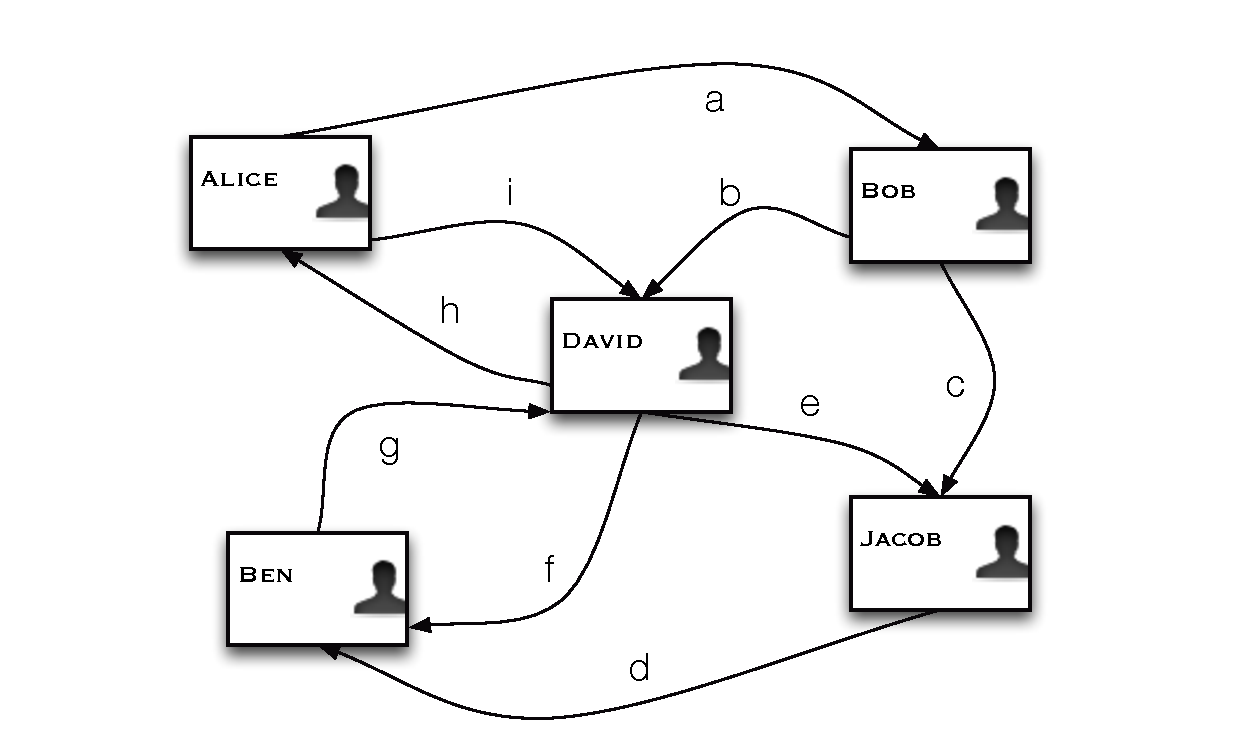
\includegraphics[scale=0.5]{./plots/motivation_1.pdf}}
	\only<2>{Alice tweets a message after World Cup final. 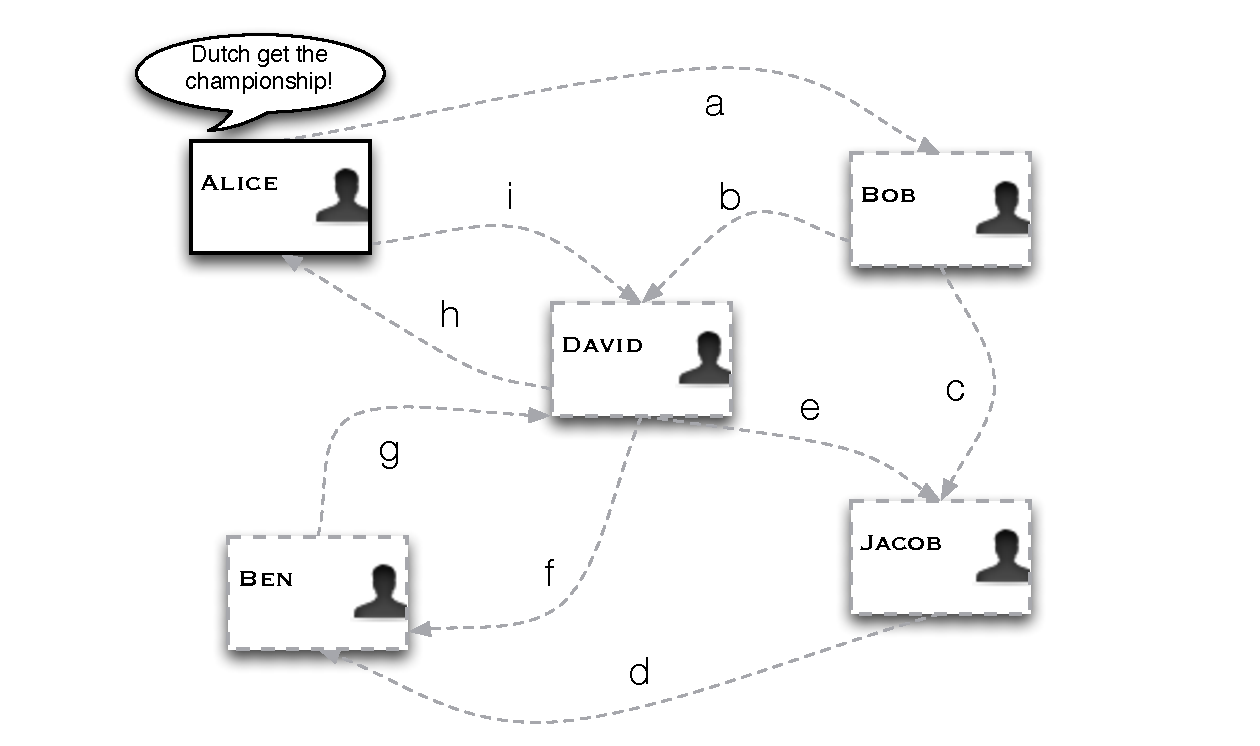
\includegraphics[scale=0.5]{./plots/motivation_2.pdf}}
	\only<3>{Bob sees the message and retweets the message from Alice. 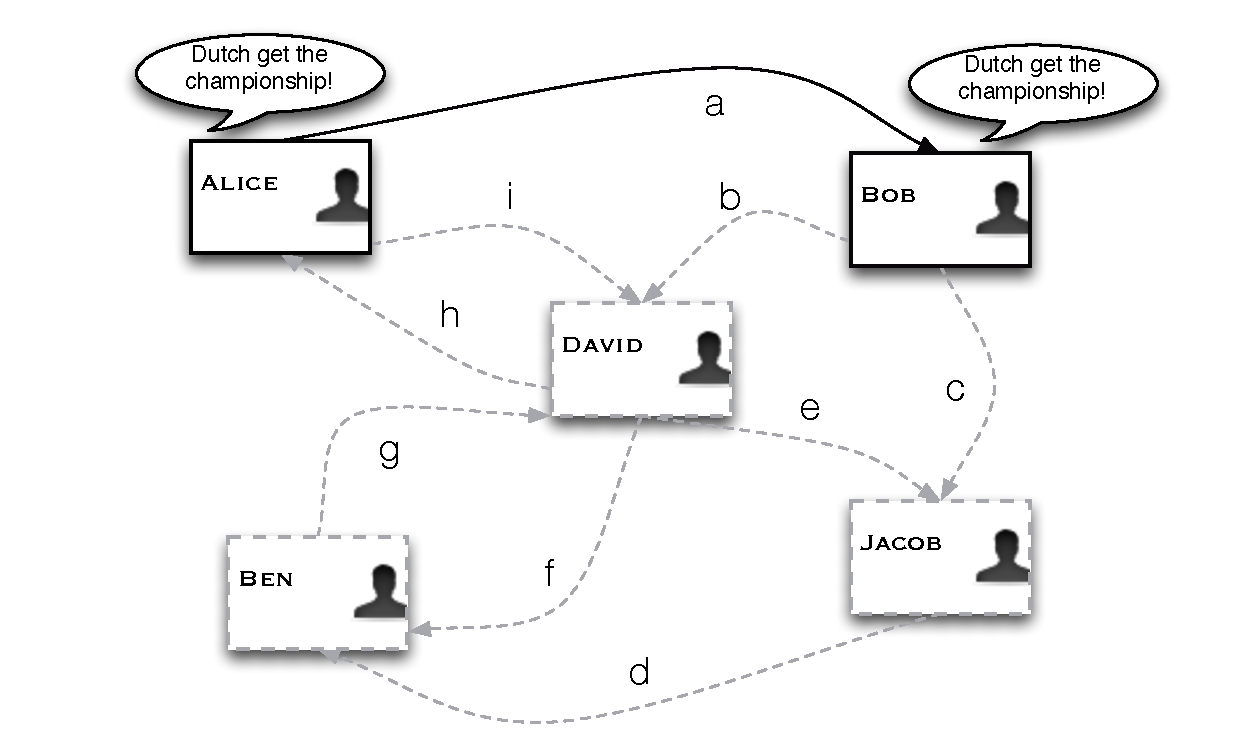
\includegraphics[scale=0.5]{./plots/motivation_3.pdf}}
	\only<4>{Jacob retweets the message from Bob. 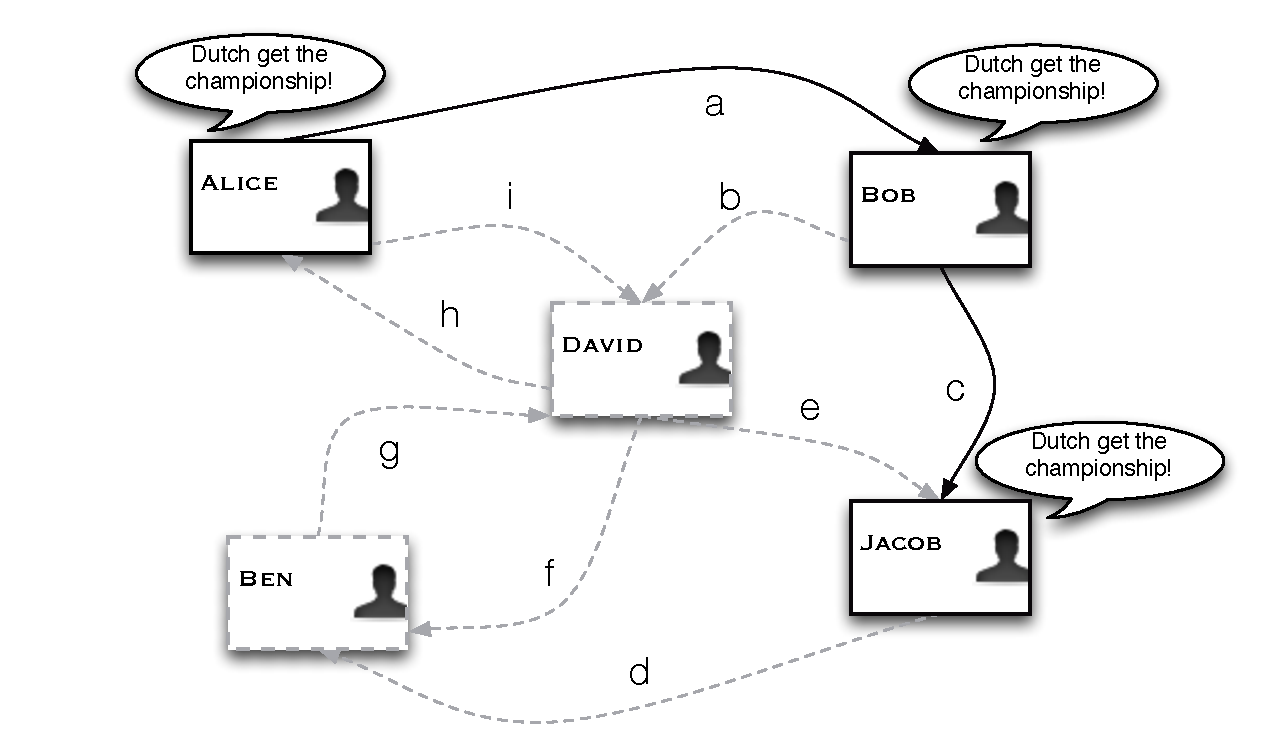
\includegraphics[scale=0.5]{./plots/motivation_4.pdf}}
	\only<5>{Ben retweets the message from Jacob. 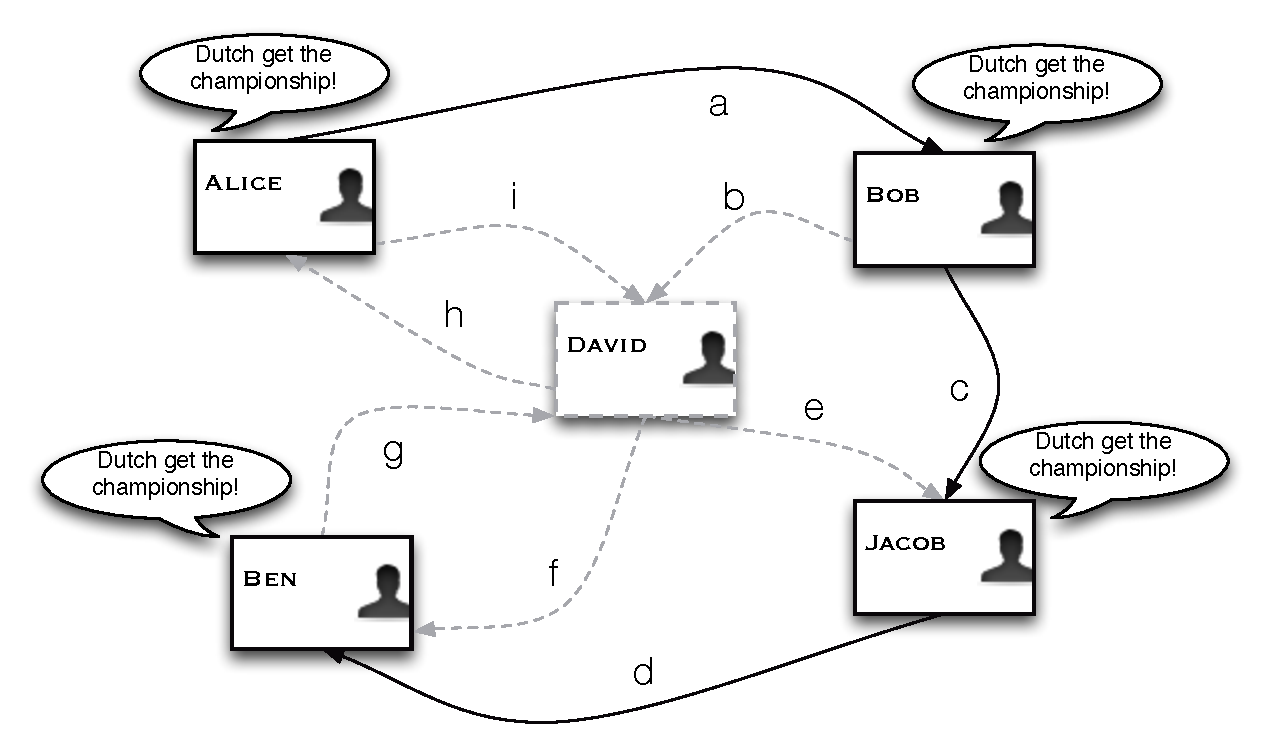
\includegraphics[scale=0.5]{./plots/motivation_5.pdf}}
	\only<6>{David does not like soccer.  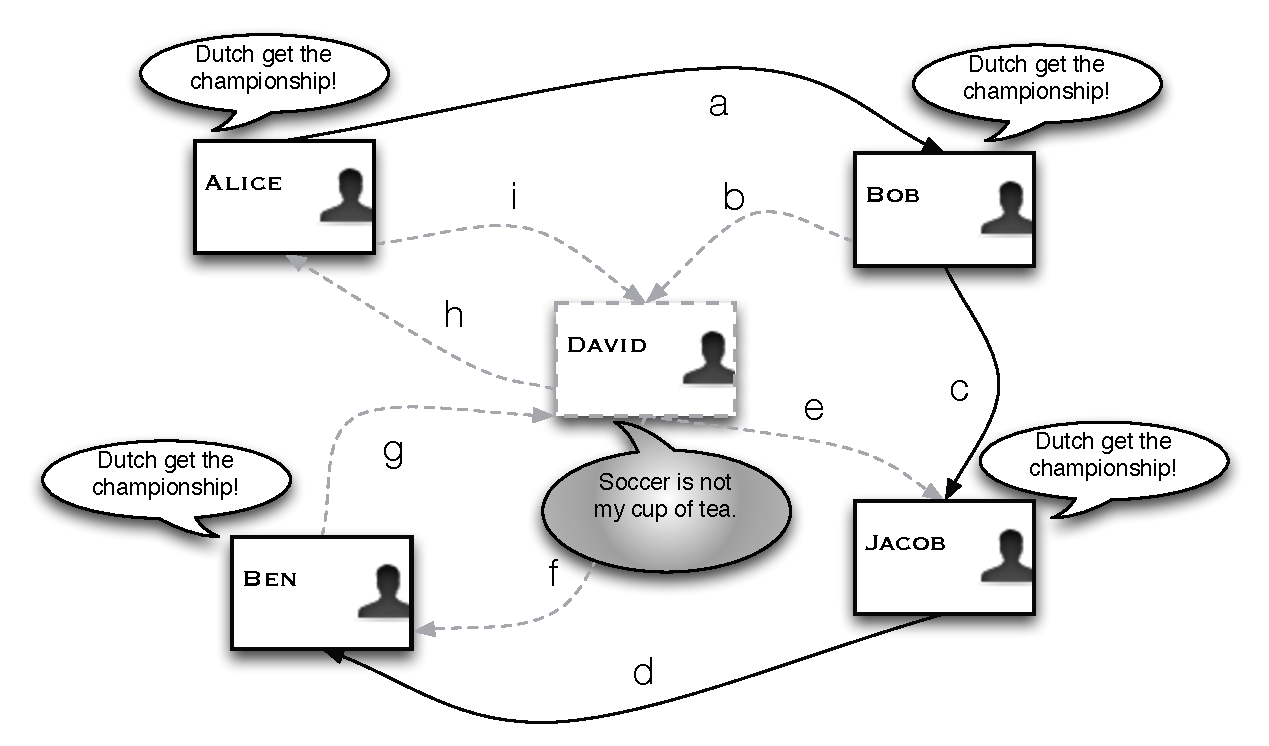
\includegraphics[scale=0.5]{./plots/motivation_6.pdf}}
\end{frame}

\begin{frame}{Network Response Problem}
	\begin{itemize}
		\item Definition:
		\begin{itemize}
			\item Given a complex network $G$, and an action $\ab$ performed on the network.
			\item Task: predict the subnetwork that responses to the action.
			\begin{itemize}
				\item Which nodes $v\in V_{\ab}$ perform the action? $V_{\ab}=\{Alice,Bob,Jacob,Ben\}$
				\item Which directed edges $e\in E_{\ab}$ relay the action from one node to its neighbors? $E_{\ab}=\{a,c,d\}$
			\end{itemize}
		\end{itemize}
	\end{itemize}
	\vspace{-10mm}
	\begin{figure}
		\center
		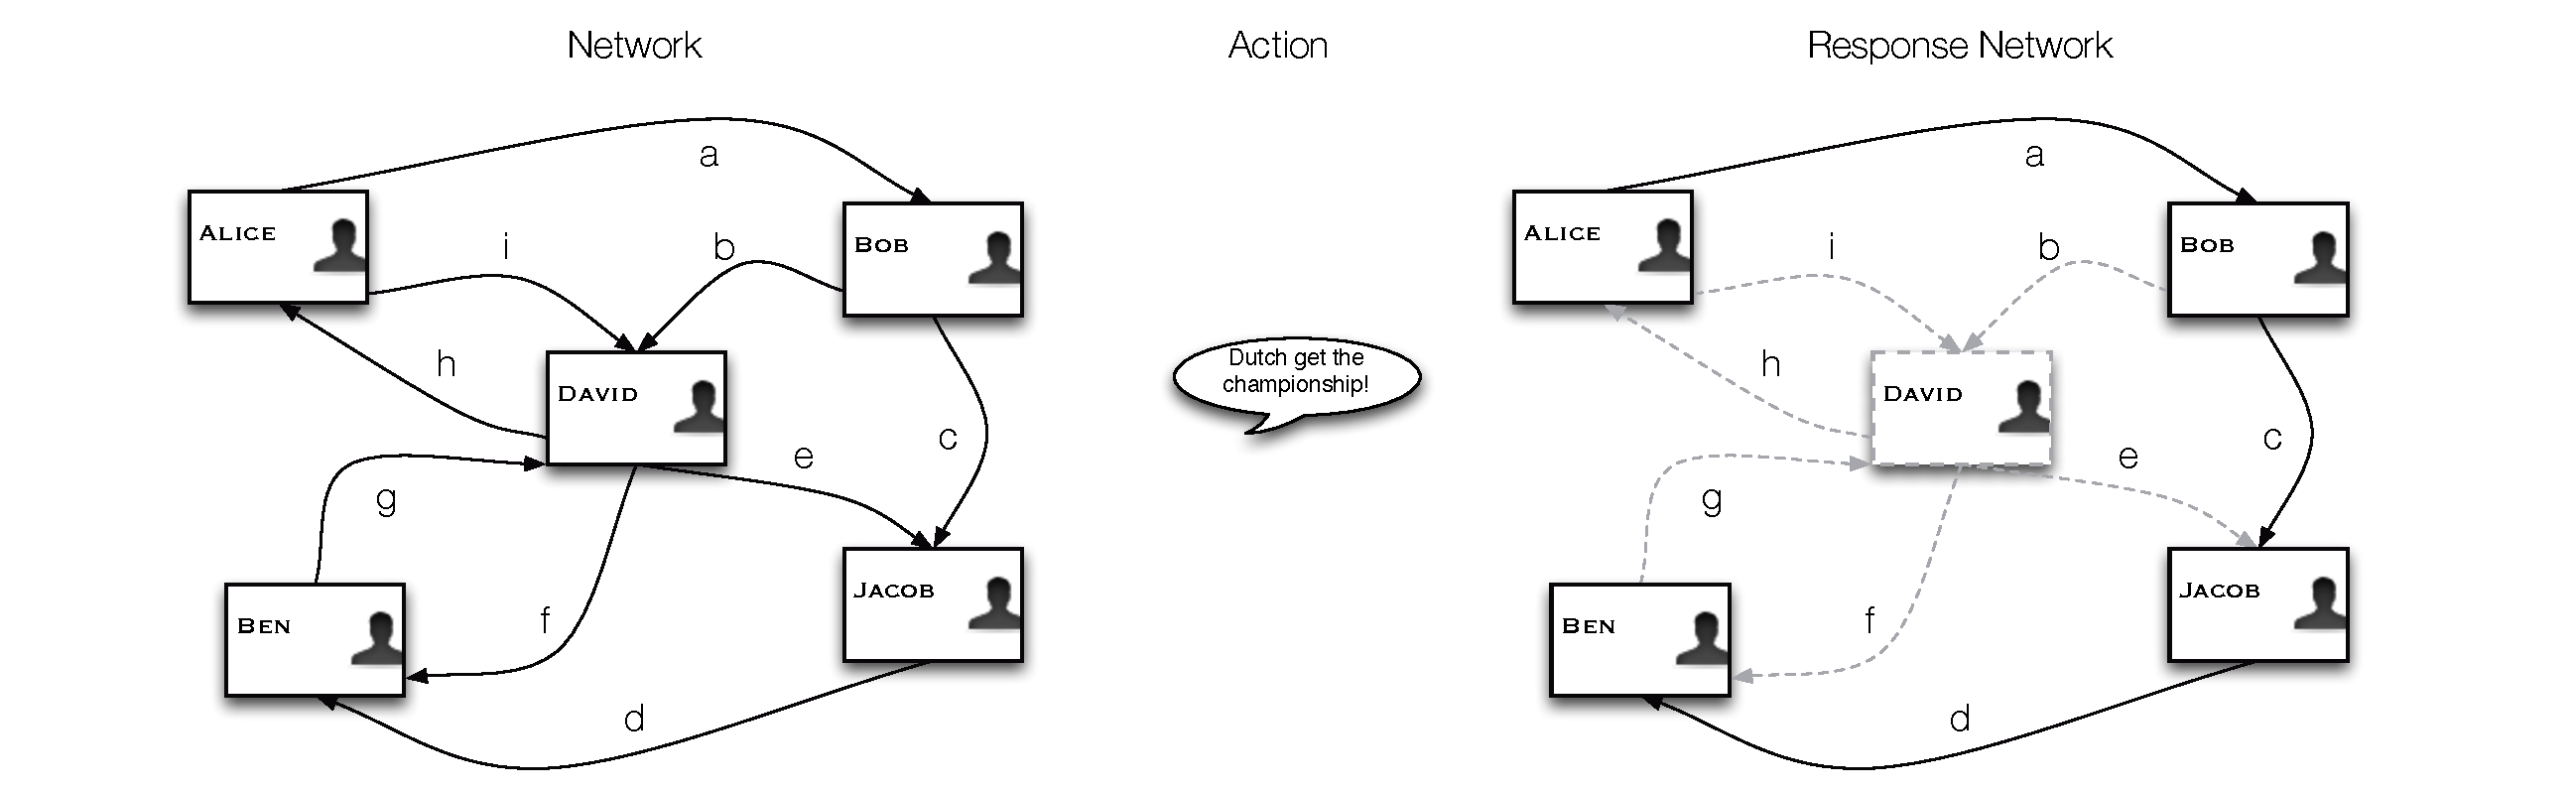
\includegraphics[scale=0.25]{./plots/problem_definition.pdf}
	\end{figure}
\end{frame}


\begin{frame}{Contributions}
	\begin{itemize}
		\item {\color{aaltoPurple} Context-sensitive prediction}. The influence from node $u$ to node $v$ not only depends on their connections but also depends on the action $\ab$ under consideration.
		\item {\color{aaltoPurple} Structure output learning}. We model the problem as predicting for each action (e.g. a tweet) a response network ({\em directed acyclic graph}).
		\item {\color{aaltoPurple} Efficient inference algorithms to discover the response network:}
		\begin{itemize}
			\item {\color{aaltoPurple} Semidefinite programming relaxation} of integer quadratic programming with approximation guarantee.
			\item {\color{aaltoPurple} Greedy algorithm} as a scalable approach.
		\end{itemize}
		\item {\color{aaltoPurple} Empirically performance} is shown to be better than the state-of-the-art.
	\end{itemize}
\end{frame}

\iffalse
\begin{frame}{Motivation}
	\begin{itemize}
		\item Our model is motivated by the following observation
		\begin{itemize}
			\item {\em\color{aaltoPurple} Context-sensitive}: The influence from node $u$ to node $v$ not only depends on their connections but also depends on the action $\ab$ under consideration.
			\item For example: $u$ and $v$ are social network friends, $v$ will direct/share the post from $u$ if it is about {\it science} but not about {\it politics}.
		\end{itemize}
		\item We approach the problem by {\em Structured Output Learning}:
		\begin{itemize}
			\item Model the response graph as a {\em directed acyclic graph} (DAG).
			\item Learn a function for mapping from action description to the response graph.
			\item Given a new action, predict the DAG that is most favourable to performing the action.
		\end{itemize}
	\end{itemize}
\end{frame}
\fi

\begin{frame}{Model}
	\begin{itemize}
		\item Model is defined on directed network.
		\begin{itemize}
			\item Any undirected network can be seen as special case by replacing undirected edges with two directed ones.
			\begin{figure}
				\center
				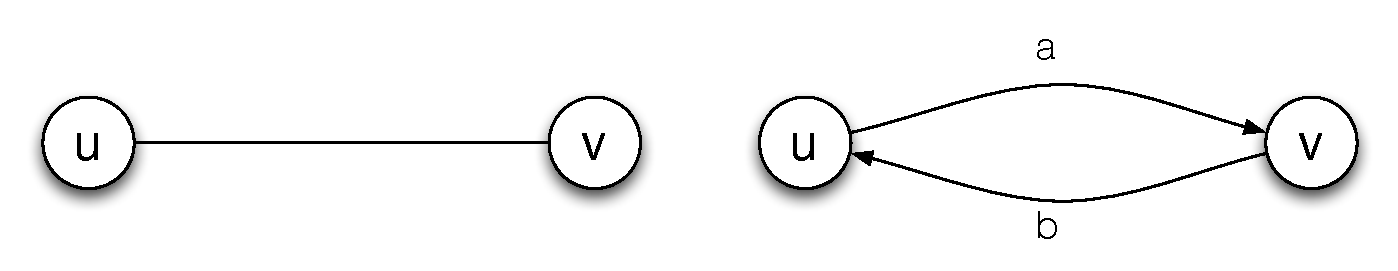
\includegraphics[scale=0.2]{./plots/model_definition.pdf}
			\end{figure}
		\end{itemize}
		\item Notation of edge labels:
		\begin{figure}
			\center
			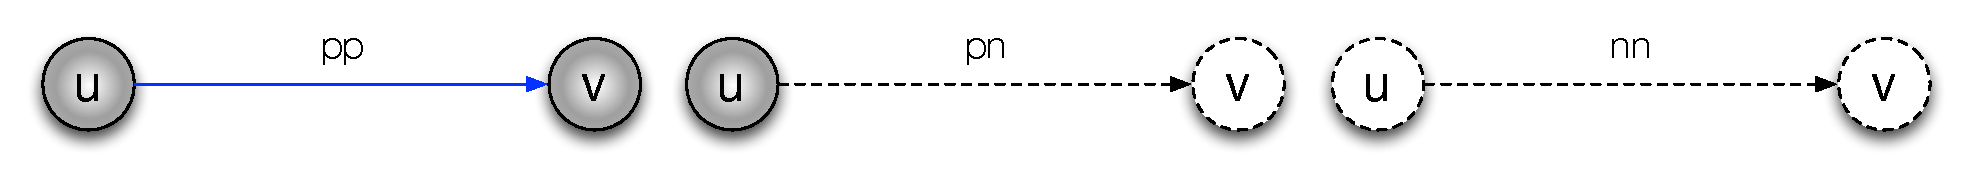
\includegraphics[scale=0.2]{./plots/notations.pdf}
		\end{figure}
		\item Feature maps:
		\begin{itemize}
			\item {\it Input feature}: Encode $\ab$ as $\phi(\ab)$ (e.g. bag-of-word of a tweet).
			\item {\it Output feature}: Encode $G_{\ab}$ as $\psi(G_{\ab})$ (e.g. a set of edges and their labels)
		\end{itemize}
	\end{itemize}
		\vspace{-6mm}
	\begin{multicols}{2}
	{\scriptsize
		\begin{align*}
			\psi(G_{\ab}) 
			&= \{a_{\pp},a_{\pn},a_{\nn},b_{\pp},b_{\pn},b_{\nn},c_{\pp},c_{\pn},c_{\nn},\cdots\}\\
			&= \{1,\quad 0,\quad 0,\quad 1,\quad 0,\quad 0,\quad 0,\quad 1,\quad 0,\cdots\}
		\end{align*}}

	\begin{figure}
		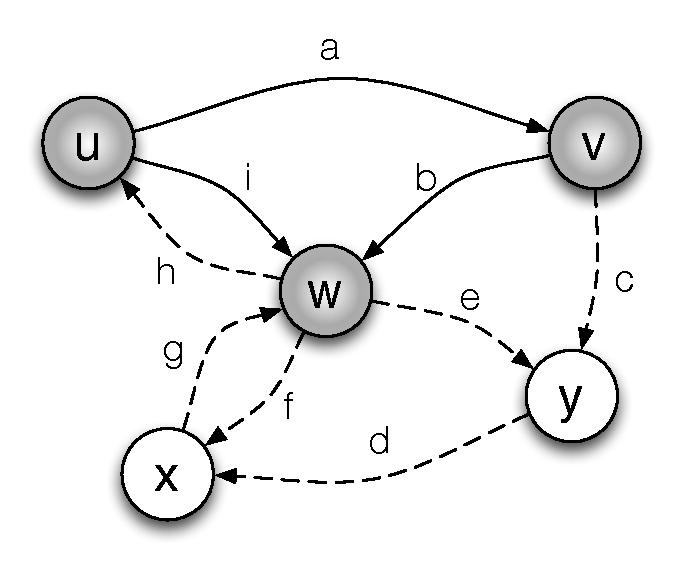
\includegraphics[scale=0.25]{./plots/propagation_example.pdf}
	\end{figure}
	\end{multicols}
\end{frame}

\begin{frame}{Structure Output Prediction Model}
	\begin{itemize}
		\item Compatibility score for $(\ab,G_{\ab})$: $F(\ab,G_{\ab},\wb) = \ip{\wb}{\varphi(\ab,G_{\ab})}$
			\begin{itemize}
				\item $\wb$ is the feature weight to be learned.
				\item $\varphi(\ab,G_{\ab})=\phi(\ab)\otimes\psi(G_{\ab})$ is joint feature map.
				\item Intuition: given an action $\ab$, the score of correct response graph $(\ab,G_{\ab})$ should be higher than any incorrect response graph $(\ab,G_{\ab}')$.
				\begin{align*}
					F(\ab,G_{\ab},\wb)>F(\ab,G_{\ab}',\wb), \quad \forall G_{\ab}'\in\Hcal(G)
				\end{align*}
			\end{itemize}
		\item $\wb$ is learned by solving structured output learning problem
		\begin{align*}
			\underset{\wb,\xi}{\minimize} &\quad \frac{1}{2}||\wb||^2_2+C\sum_{i=1}^{m}\xi_i \\
			\textbf{s.t.} &\quad F(a_i,G_{\ab_i};\wb) > \underset{G_{\ab_i}'\in\Hcal(G)}{\maximize} (F(a_i,G_{\ab_i}',\wb)\\
			&\quad +\ell_G(G_{\ab_i},G_{\ab_i}'))-\xi_i, \xi_i\ge 0,\forall i\in\{1,\cdots,m\},
		\end{align*}
	\end{itemize}
\end{frame}

\begin{frame}{Inference Problem}
	\begin{itemize}
		\item To solve the optimization, we have to solve similar inference problem appeared both in training and in prediction.
		\item In prediction phase:
		\begin{itemize}
			\item Given the feature weight $\wb$ and the complex network $G$.
			\item To find out a network $H^*=(V_H,E_H)$ that gives the maximal compatibility score for a given action $\ab$
		\end{itemize}
	\end{itemize}
	\only<1>{
	\scriptsize{
	\begin{align*}
		H^*(a) 
		&= \underset{H\in \Hcal({\color{aaltoRed}G})}{\argmax}\, F({\ab},H;{\color{aaltoRed}\wb}) \nonumber\\
		&= {\color{aaltoGray}\underset{H\in \Hcal(G)}{\argmax}\, \ip{\wb}{\phi(a)\otimes\psi(H)}} \nonumber\\
		&= {\color{aaltoGray}\underset{H\in \Hcal(G)}{\argmax}\, \sum_{e\in E^H}s_{\yb_e}(e,a,\wb)} 
	\end{align*}
	}}
	\only<2>{
	\scriptsize{
	\begin{align*}
		H^*(a) 
		&= \underset{H\in \Hcal({\color{aaltoRed}G})}{\argmax}\, F({\color{aaltoPurple}\ab},H;{\color{aaltoRed}\wb}) \nonumber\\
		&= {\color{aaltoGray}\underset{H\in \Hcal(G)}{\argmax}\, \ip{\wb}{\phi(a)\otimes\psi(H)}} \nonumber\\
		&= {\color{aaltoGray}\underset{H\in \Hcal(G)}{\argmax}\, \sum_{e\in E^H}s_{\yb_e}(e,a,\wb)} 
	\end{align*}
	}}
	\only<3>{
	\scriptsize{
	\begin{align*}
		H^*(a) 
		&= \underset{{\color{aaltoBlue}H}\in \Hcal({\color{aaltoRed}G})}{\argmax}\, F({\color{aaltoPurple}\ab},{\color{aaltoBlue}H};{\color{aaltoRed}\wb}) \nonumber\\
		&= {\color{aaltoGray}\underset{H\in \Hcal(G)}{\argmax}\, \ip{\wb}{\phi(a)\otimes\psi(H)}} \nonumber\\
		&= {\color{aaltoGray}\underset{H\in \Hcal(G)}{\argmax}\, \sum_{e\in E^H}s_{\yb_e}(e,a,\wb)} 
	\end{align*}
	}}
	\only<4>{
	\scriptsize{
	\begin{align*}
		H^*(a) 
		&= {\color{aaltoGray}\underset{{\color{aaltoBlue}H}\in \Hcal({\color{aaltoRed}G})}{\argmax}\, F({\color{aaltoPurple}\ab},{\color{aaltoBlue}H};{\color{aaltoRed}\wb})} \nonumber\\
		&= {\underset{H\in \Hcal(G)}{\argmax}\, \ip{\wb}{\phi(a)\otimes\psi(H)}} \nonumber\\
		&= {\color{aaltoGray}\underset{H\in \Hcal(G)}{\argmax}\, \sum_{e\in E^H}s_{\yb_e}(e,a,\wb)} 
	\end{align*}
	}}
	\only<5>{
	\scriptsize{
	\begin{align*}
		H^*(a) 
		&= {\color{aaltoGray}\underset{{\color{aaltoBlue}H}\in \Hcal({\color{aaltoRed}G})}{\argmax}\, F({\color{aaltoPurple}\ab},{\color{aaltoBlue}H};{\color{aaltoRed}\wb})} \nonumber\\
		&= {\color{aaltoGray}\underset{H\in \Hcal(G)}{\argmax}\, \ip{\wb}{\phi(a)\otimes\psi(H)}} \nonumber\\
		&= {\underset{H\in \Hcal(G)}{\argmax}\, \sum_{e\in E^H}s_{\yb_e}(e,a,\wb)}
	\end{align*}
	}}

\end{frame}

\begin{frame}{$NP$-hardness}
	\begin{align}
		H^*(a) 
		%&= \underset{H\in \Hcal(G)}{\argmax}\, F({\ab},{H};{\wb}) \nonumber\\
		%&= \underset{H\in \Hcal(G)}{\argmax}\, \ip{\wb}{\phi(a)\otimes\psi(H)} \nonumber\\
		&= \underset{H\in \Hcal(G)}{\argmax}\, \sum_{e\in E^H}s_{\yb_e}(e,a,\wb) \label{inference}
	\end{align}
	\begin{lemma}
		Finding the graph that maximizes Eq.~(\ref{inference}) is an $\mathcal{NP}$-hard problem.
	\end{lemma}
	\begin{proof}
		Reduction from {\sc max-cut} problem.
	\end{proof}
\end{frame}

\iffalse
\vspace{-8mm}
\begin{figure}
	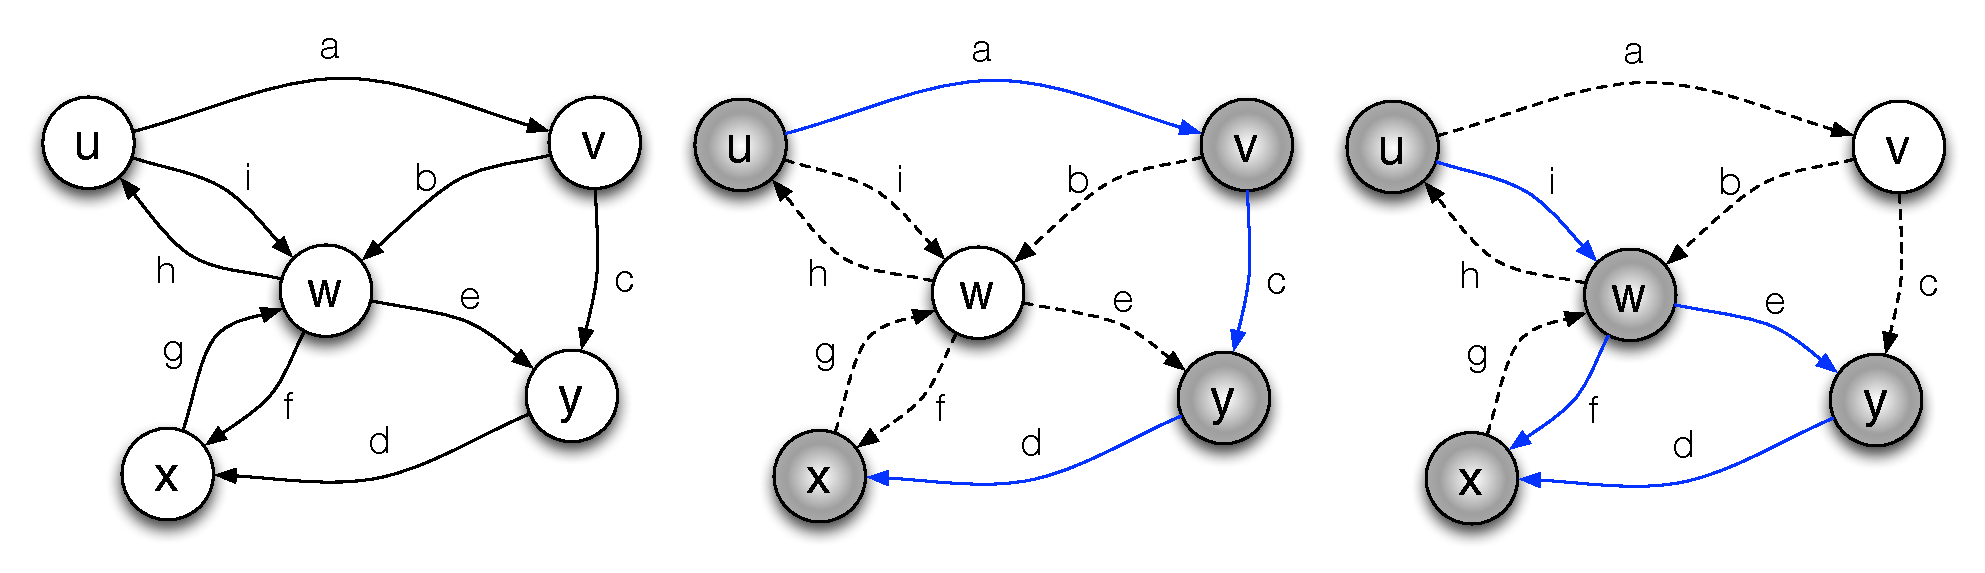
\includegraphics[scale=0.25]{./plots/inference_problem.pdf}
	\put(-230,65){{\tiny $\{s_{\pp}(a,\ab,\wb),s_{\pn}(a,\ab,\wb)\}$}}
	\put(-130,65){{\tiny $s_{\pp}(a,\ab,\wb)$}}
	\put(-50,65){{\tiny $s_{\pn}(a,\ab,\wb)$}}
\end{figure}
\fi

\iffalse
\begin{frame}{Inference Problem in Two Modes}
	\begin{itemize}
		\item The inference problem can be address into two modes based on the values of edge labels $\yb_e$.
		\begin{itemize}
			\item {\it Activation mode}: $\yb_e\in\{\pp,\pn\}$
			\item {\it Negative-feed mode}: $\yb_e\in\{\pp,\pn,\nn\}$
		\end{itemize}
	\end{itemize}
	\begin{figure}
		\centering
		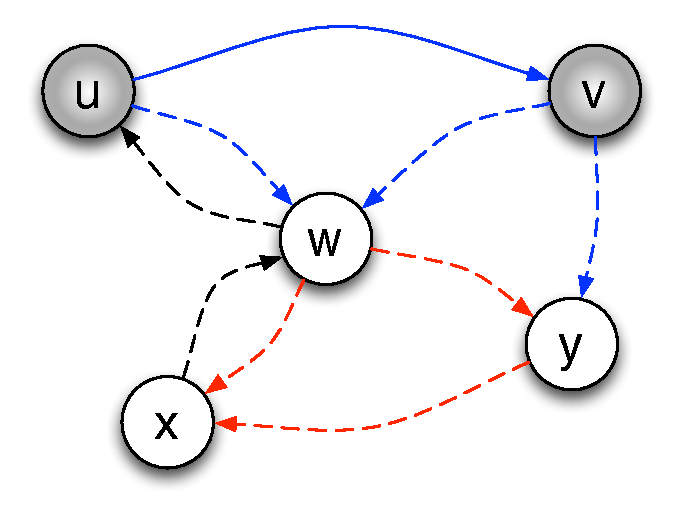
\includegraphics[scale=0.35]{./plots/two_modes.pdf}
		\put(-60,85){\pp}
		\put(-75,65){\pn}
		\put(-50,65){\pn}
		\put(-25,50){\pn}
		\put(-45,35){\nn}
		\put(-70,25){\nn}
		\put(-55,20){\nn}
	\end{figure}
\end{frame}
\fi

\begin{frame}[allowframebreaks]{Approximate Inference through {\sc SDP} relaxation}
	\begin{itemize}
		\item {{\sc sdp} inference}:
		\begin{itemize}
			\item We formulate the inference problem as {\it integer quadratic programming} ({\sc iqp}).
			\begin{itemize}
				\item Introduce for each node $u\in V$ a binary variable $x_u\in\{-1,+1\}$.
				\item Introduce a special variable $x_0\in\{-1,+1\}$ to distinguish activated node.
			\end{itemize}
			{\scriptsize
			\begin{align*}
			\maximize \; \frac{1}{4} \sum_{(u, v)\in E}\, [ & s_{\pn}(u,v) (1 + x_0 x_u - x_0 x_v - x_u x_v)  \\ 
				+ & s_{\nn}(u,v) (1 - x_0 x_u - x_0 x_v + x_u x_v)  \\ 
				+ & s_{\pp}(u,v) (1 + x_0 x_u + x_0 x_v + x_u x_v) ] \\
			\textbf{s.t.} \quad  x_0, x_u, x_v &\in \{-1,+1\}, \text{ for all } u,v\in V,
			\end{align*}}
			\item {\sc iqp} is solved by {\it semidefinite programming relaxation} ({\sc sdp}).
			\item Optimization guarantee $E[Z] \ge (\alpha-\epsilon) Z_{R} $ with $\alpha>0.796$, $Z$ is objective achieved by {\sc sdp}, $Z_R$ is objective of {\sc iqp}.
		\end{itemize}
	\end{itemize}
\end{frame}

\begin{frame}{{\sc greedy} Inference}
	\begin{itemize}
		\item {{\sc greedy} inference}:		
		\begin{itemize}
			\item We have shown that the inference problem can be expressed equivalently as nodes and their scores
			{\scriptsize
			\begin{align*}
				H^{*}(\ab) = \underset{{H \in {\cal H}(G)}}{\argmax}\,\sum_{ \substack{v_i\in V^H_p}}F_m(v_i).
			\end{align*}}
			\item The greedy algorithm iteratively maximizes the equation by adding one node into activited node set $V_p^H$ in each iteration.
			\item The time complexity for greedy inference algorithm is $\Theta(|E|\log|V|)$.
			\item We are able to run {\sc greedy} algorithm on network with upto $2000$ nodes.
		\end{itemize}
	\end{itemize}
\end{frame}


\iffalse
\begin{frame}{Comparison of Inference Algorithms}
	\begin{itemize}
		\item Experiment settings:
			\begin{itemize}
				\item Given an action $\ab\in\Acal$, we use 'SPIN' with different inference algorithms to predict response network $G_{\ab}$.
			\end{itemize}
		\item Result:
			\begin{table}[t]
			\scriptsize
			\centering
			\begin{tabular}{|p{8.5mm}|p{7mm}p{8mm}p{8mm}|p{7mm}p{8mm}p{10mm}|}
			  \hline
			\multirow{2}{*}{\textbf{Data}} & \multicolumn{3}{c}{\textbf{Accuracy}}  & \multicolumn{3}{|c|}{\textbf{ Time ({\tiny$10^2$s})}} \\ \cline{2-7}
			 & \scriptsize{SDP} & \scriptsize{Greedy Neg} & \scriptsize{Greedy Act}  & \scriptsize{SDP} & \scriptsize{Greedy Neg} & \scriptsize{Greedy Act} \\ \hline
			S100  & \textbf{79.9} & \em{77.6} & {72.9}  & {16.0} & \em{1.5} & \textbf{0.2} \\
			M100  & \textbf{75.8} & \em{73.6} & {68.5}  & {15.2} & \em{1.4} & \textbf{0.2} \\
			L100  & \textbf{75.1} & \em{72.0} & {67.4}  & {13.7} & \em{1.6} & \textbf{0.3} \\ \hline
			\textbf{Geom.} & \textbf{76.9} & \em{74.3} &  {69.6} & {15.0} & \em{1.5} & \textbf{0.3} \\
			\hline
			\end{tabular}
			\end{table}
	\end{itemize}
\end{frame}
\fi

\begin{frame}{Experiment: Context-sensitive Prediction}
	\begin{itemize}
		\item Experiment settings:
			\begin{itemize}
				\item We assume action is known (e.g. bag-of-word of a tweet).
				\item Task is to predict the response network given an action.
				%\item {\em Predicted Subgraph Coverage} (PSC) is defined as $\mathrm{PSC}=\frac{1}{mn} \sum_{i=1}^{m} \sum_{v\in V_i} |G_v|$.
				\item {\em Predicted Subgraph Coverage} (PSC) is the relative size of correctly predicted subgraph in terms of node labels.)
			\end{itemize}
		\item Result:
		\begin{table}[t]
		\scriptsize
		\centering
		\begin{tabular}{|@{ }c@{ }|@{}c@{ }c@{ }c@{}|@{}c@{ }c@{ }c@{}|@{}c@{ }c@{}|@{}c@{ }c@{ }c@{}|}
		  \hline
		\multirow{2}{*}{\textbf{Dataset}} & \multicolumn{3}{c}{\textbf{Node Accuracy}} & \multicolumn{3}{|c}{\textbf{Node $F_1$ Score}} & \multicolumn{2}{|c}{\textbf{Edge Acc}} & \multicolumn{3}{|c|}{{\em PSC}}  \\ \cline{2-12}
		 & \scriptsize{SVM} & \scriptsize{MMCRF} & \scriptsize{SPIN} & \scriptsize{SVM} & \scriptsize{MMCRF} & \scriptsize{SPIN} & \scriptsize{SVM}  & \scriptsize{SPIN}  & \scriptsize{SVM} & \scriptsize{MMCRF} & \scriptsize{SPIN}  \\ \hline
		   memeS  & \textbf{73.4} & {68.0} & \em{72.2} & {39.0} & \em{39.8} & \textbf{47.1} & \textbf{62.7} & {45.6} & {23.4} & \em{25.3} & \textbf{33.6} \\ 
		   memeM  & \textbf{82.1} & {79.0} & \em{81.5} & {29.1} & \em{30.1} & \textbf{38.0} & {61.1} & \textbf{68.8} & {18.6} & \em{18.8} & \textbf{28.3} \\ 
		   memeL  & \textbf{89.9} & {88.3} & \em{89.8} & {26.7} & \em{27.1} & \textbf{35.0} & {45.5} & \textbf{80.0} & {17.7} & \em{18.9} & \textbf{27.6} \\ 
		%M100  & {71.2} & \em{73.6} & \textbf{76.7} & {49.3} & \em{50.8} & \textbf{54.3} & {33.3} & \textbf{61.7} & {33.3} & \textbf{35.6} & \em{34.6} & \textbf{0.1} & {0.2} & \textbf{0.1}\\ 
		%M500  & {89.0} & \em{91.4} & \textbf{92.0} & \textbf{18.8} & {13.5} & \em{14.6} & {28.2} & \textbf{92.6} & \em{29.3} & {26.4} & \textbf{29.5} & {9.0} & \em{3.8} & \textbf{3.2}\\ 
		M700  & {91.9} & \textbf{94.1} & \em{92.1} & \em{13.8} & {7.3} & \textbf{14.2}  & {26.3} & \textbf{93.0} & \em{29.4} & {23.9} & \textbf{34.4} \\ 
		M1k & {94.1} & \textbf{95.8} & \em{94.2} & \textbf{10.9} & {3.5} & \em{9.3}   & {26.6} & \textbf{94.7} & \em{33.7} & {16.6} & \textbf{35.2} \\ 
		M2k & \em{96.8} & \textbf{97.6} & {96.7} & \textbf{6.2} & {1.4} & \em{3.4}    & {25.3} & \textbf{97.6} & \textbf{34.6} & {9.6} & \em{14.7} \\ 
		%L100  & {69.4} & \em{72.2} & \textbf{75.7} & {51.1} & \em{53.1} & \textbf{57.4} & {31.6} & \textbf{62.3} & {30.9} & \em{31.7} & \textbf{33.4} & \textbf{0.1} & \em{0.2} & {0.3}\\ 
		%L500  & {85.9} & \textbf{89.1} & \em{86.8} & \em{21.7} & {15.1} & \textbf{24.7} & {27.9} & \textbf{87.9} & \em{14.2} & {11.2} & \textbf{19.7} & {6.5} & \em{3.2} & \textbf{2.1}\\ 
		L700  & {89.7} & \textbf{92.4} & \em{89.7} & \em{16.2} & {9.4} & \textbf{17.3}  & {26.5} & \textbf{90.4} & \em{9.5} & {6.7} & \textbf{12.5} \\ 
		L1k & \em{92.4} & \textbf{94.4} & {91.5} & \em{12.4} & {6.4} & \textbf{13.9}  & {26.4} & \textbf{92.3} & \em{6.1} & {4.4} & \textbf{8.4} \\ 
		L2k & \em{92.5} & \textbf{94.5} & {91.9} & \em{12.3} & {5.4} & \textbf{12.7}  & {26.5} & \textbf{93.2} & \em{6.0} & {2.9} & \textbf{7.2} \\ \hline
		\textbf{Geom.}  & {85.5} & \em{86.4} & \textbf{86.6} & \em{19.8} & {12.6} & \textbf{20.3} & {32.6} & \textbf{79.7} & \em{18.9} & {14.2} & \textbf{21.7} \\
		\hline
		\end{tabular}
		\label{table_global_res_svm}
		\end{table}
	\end{itemize}
\end{frame}

\begin{frame}{Experiment: Context-free Prediction}
	\begin{itemize}
		\item Experiment settings:
			\begin{itemize}
				\item We assume action is unknown.
				\item Task is to predict directed edges from a cascade of actions and compare the results against other influence network prediction methods.
				\item The measure of success is {\em Precision@$K$}, where we ask for top-$K$ percent edge predictions and compute the precision.
			\end{itemize}
		\item Result:
			\begin{table}[t]
			\scriptsize
			\centering
			\begin{tabular}{|@{ }c@{ }|@{ }c@{ }|@{ }c@{ }|@{ }c@{ }|@{ }c@{ }|@{ }c@{ }|@{ }c@{ }|@{ }c@{ }|@{ }c@{ }|}
			  \hline
			\multirow{2}{*}{\textbf{Dataset}} & \multirow{2}{*}{\textbf{Model}} & \multirow{2}{*}{\textbf{T ({\tiny$10^3$s})}} & \multicolumn{6}{c|}{Precision @ $K$} \\ \cline{4-9}
			 & & & {$10\%$} & {$20\%$} & {$30\%$} & {$40\%$} & {$50\%$} & {$60\%$} \\ \hline
			\multirow{3}{*}{\textbf{memeS}}
			& SPIN & \em{5.50} & \textbf{82.9} & \textbf{81.0} & \textbf{76.0} & \textbf{74.0} & \textbf{74.0} & \textbf{70.0}  \\  
			& ICM-EM & \textbf{0.01} & {60.3} & {63.5} & {65.1} & {62.0} & {62.0} & {61.5}  \\ 
			& NETRATE & {5.83} & \em{76.2} & \em{73.8} & \em{70.4} & \em{68.7} & \em{68.7} & \em{66.8} \\ \hline 
			\multirow{3}{*}{\textbf{memeM}}
			& SPIN & \em{5.52} & \textbf{82.7} & \textbf{72.1} & \textbf{70.5} & \textbf{69.2} & \textbf{69.2} & \textbf{67.9}  \\  
			& ICM-EM & \textbf{0.02} & {56.3} & {55.3} & {56.8} & {57.4} & {57.4} & {56.3}  \\ 
			& NETRATE & {13.93} & \em{61.2} & \em{64.6} & \em{62.9} & \em{62.5} & \em{62.5} & \em{62.4}  \\ \hline 
			\multirow{3}{*}{\textbf{memeL}}
			& SPIN & \em{4.75} & \textbf{82.2} & \textbf{73.6} & \textbf{69.1} & \textbf{66.7} & \textbf{66.7} & \textbf{65.9}  \\  
			& ICM-EM & \textbf{0.01} & {52.1} & {55.7} & {54.2} & {56.5} & {56.5} & {56.7}  \\ 
			& NETRATE & {12.63} & \em{56.5} & \em{57.8} & \em{60.0} & \em{59.3} & \em{59.3} & \em{59.4}  \\ \hline
			\end{tabular}
			\end{table}
	\end{itemize}
\end{frame}

\begin{frame}{Conclusion}
	\begin{itemize}
		\item We have developed a structured output learning approach for network response prediction problem.
		\item To outperform competing methods, our model takes the advantage of two sources of prior knowledge:
		\begin{itemize}
			\item The context given by the action descriptions.
			\item The structure of an underlying network (e.g. followership in Twitter, friendship in Facebook).
		\end{itemize}
		\item The inference problem is $\mathcal{NP}$-hard, and is in practice tackled by two algorithms:
		\begin{itemize}
			\item {\sc sdp} relaxation with approximation guarantee.
			\item a fast {\sc greedy} heuristics.
		\end{itemize}
	\end{itemize}
\end{frame}

\begin{frame}{}
	
	\begin{itemize}
		%\item Poster No. 565 tonight.
		\item Thank you !
	\end{itemize}
\end{frame}

\iffalse
\begin{frame}[allowframebreaks]{Bibliography}
	%\bibliographystyle{plain}
	\bibliographystyle{apalike}
	\bibliography{example}
\end{frame}
\fi


\end{document}
